\documentclass[border=2pt]{standalone}
\usepackage{pgfplots}
\usepgfplotslibrary{statistics}
\pgfplotsset{width=7cm,compat=1.18}
\begin{document}
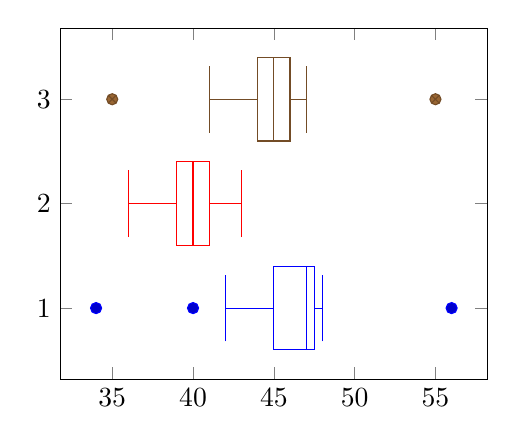
\begin{tikzpicture}
\begin{axis}
    \addplot+ [
        boxplot prepared={
            lower whisker=42, lower quartile=45,
            median=47,
            upper quartile=47.5, upper whisker=48,
        },
    ] table [row sep=\\,y index=0] { 40\\ 34\\ 56\\ };

    \addplot+ [
        boxplot prepared={
            lower whisker=36, lower quartile=39,
            median=40,
            upper quartile=41, upper whisker=43,
        },
    ]
        % no outliers:
        coordinates {};

    \addplot+ [
        boxplot prepared={
            lower whisker=41, lower quartile=44,
            median=45,
            upper quartile=46, upper whisker=47,
        },
    ] coordinates {(0,35) (0,55)};
\end{axis}
\end{tikzpicture}
\end{document}
